% Компіляція: lualatex -shell-escape main.tex (двічі)
\documentclass[12pt,a4paper]{article}

\usepackage{fontspec}
\usepackage{polyglossia}
\setdefaultlanguage{ukrainian}
\setmainfont{NewComputerModern10}
\setsansfont{Noto Sans}
\setmonofont{Noto Sans Mono}[Scale=0.82,ItalicFont={Noto Sans Mono},ItalicFeatures={FakeSlant=0.2}]

\usepackage{amsmath,amssymb,array,booktabs,caption,enumitem,float,geometry,graphicx,microtype,titlesec,xcolor}
\geometry{left=2cm,right=2cm,top=2cm,bottom=2cm}
\setlength{\parindent}{1.25cm}
\linespread{1.08}
\titleformat{\section}{\normalfont\fontsize{14}{16}\selectfont\bfseries}{\thesection}{0.6em}{}
\titleformat{\subsection}{\normalfont\fontsize{12}{14}\selectfont\bfseries}{\thesubsection}{0.6em}{}
\titlespacing*{\section}{0pt}{1.4em}{0.65em}
\titlespacing*{\subsection}{0pt}{1.1em}{0.45em}
\captionsetup{font=small,labelfont=bf,labelsep=endash}
\captionsetup[table]{position=bottom,skip=5pt}

\usepackage[newfloat]{minted}
\SetupFloatingEnvironment{listing}{name=Лістинг}
\setminted{fontsize=\scriptsize,linenos,breaklines,breakanywhere,autogobble,frame=single,framesep=2mm,bgcolor=gray!5,tabsize=4}

\usepackage[unicode,colorlinks=true,linkcolor=black,urlcolor=blue,
  pdftitle={ІО-41, Давидчук Артем, Вступ до штучного інтелекту, Лабораторна робота №3},
  pdfauthor={Давидчук Артем},pdfsubject={Агенти на основі знань}]{hyperref}

\begin{document}
\pagenumbering{gobble}
\begin{titlepage}
  \begin{center}
    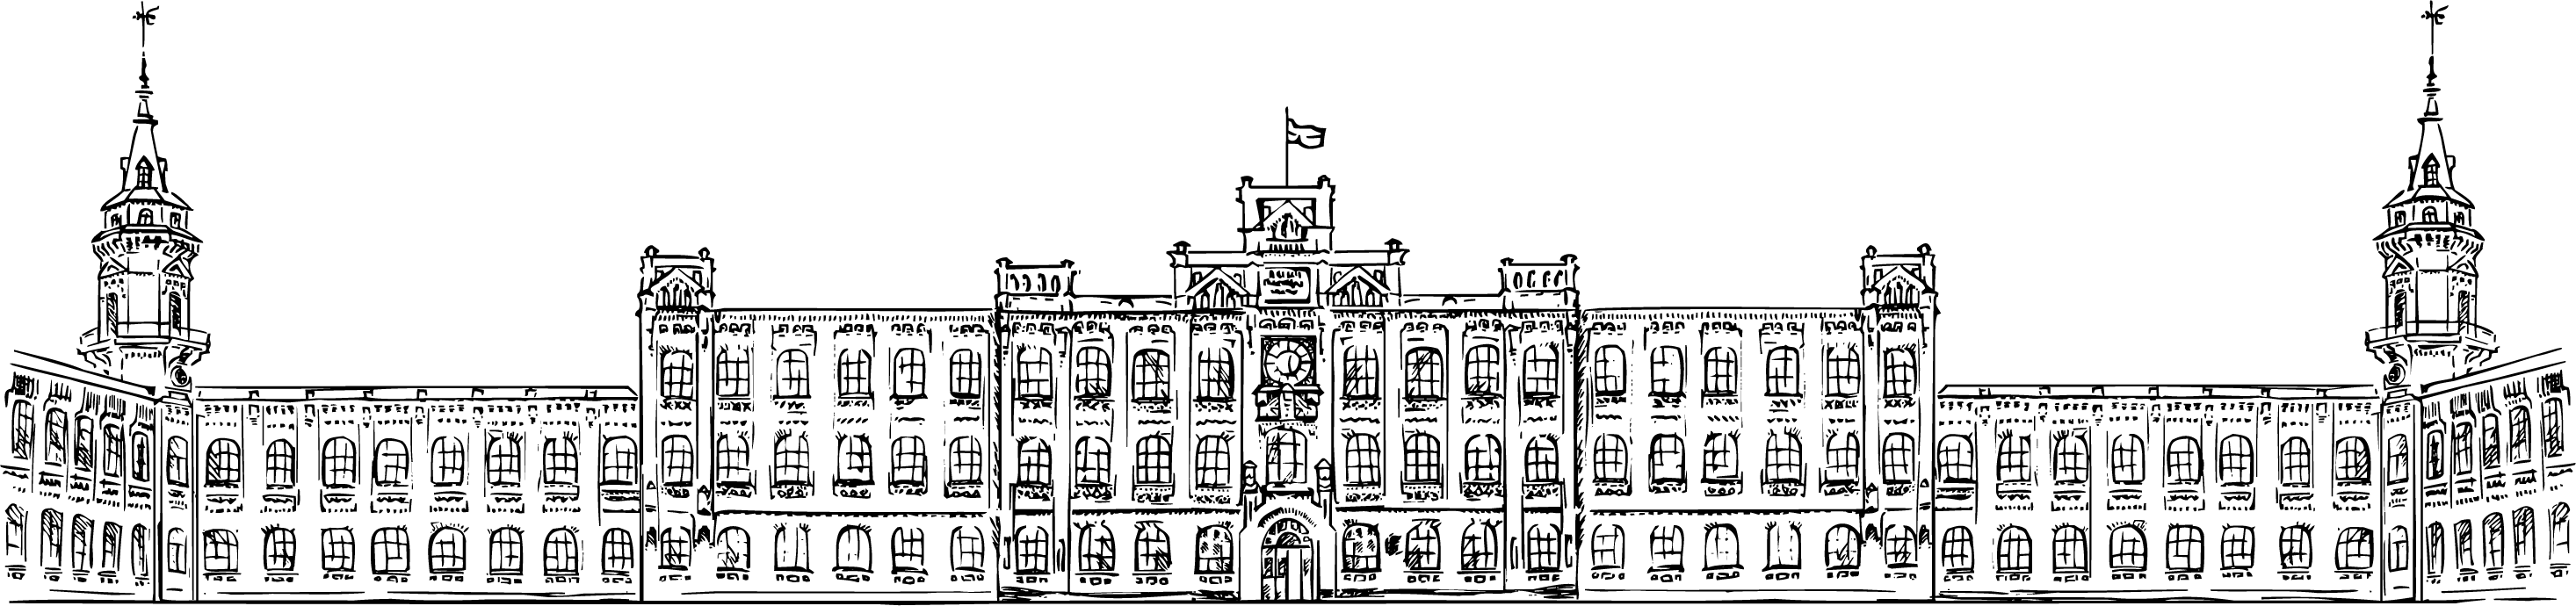
\includegraphics[width=0.7\textwidth]{../../../../../../templates/letterhead.png}
  \end{center}
  \begin{center}
    \large
    Національний технічний університет України\\
    «Київський політехнічний інститут імені Ігоря Сікорського»\\[1em]
    Факультет інформатики та обчислювальної техніки\\
    Кафедра обчислювальної техніки
  \end{center}
  \vfill
  \begin{center}
    \textbf{\LARGE Вступ до штучного інтелекту}\\[2em]
    \textbf{\Large Лабораторна робота №3}\\[0.7em]
    \parbox{0.9\textwidth}{\centering «Агенти на основі знань»}
  \end{center}
  \vfill
  \begin{flushright}
    \begin{minipage}{0.48\textwidth}
      Виконав: студент групи ІО-41\\
      \textit{Давидчук Артем}\\[1em]
      Перевірив: \textit{Кочура Ю. П.}
    \end{minipage}
  \end{flushright}
  \vfill
  \begin{center}Київ --- 2026\end{center}
\end{titlepage}
\pagenumbering{arabic}

\section{Мета роботи}

Удосконалити мережевого контролера з лабораторної роботи №2 так, щоб він
створював і використовував власну базу знань про стан каналів мережі для
побудови маршруту. Дослідити вплив накопичення знань на якість маршруту та
кількість зайвих повернень.

\section{Постановка задачі}

За основу взято зважений граф із лабораторної роботи №1. Вершини графа є
мережевими вузлами, ребра --- каналами зв'язку, а вага ребра відповідає
затримці передавання даних.

Контролер працює як агент на основі знань. Під час перебування на вузлі він
отримує не тільки локальну таблицю каналів, а й анонси про канали сусідніх
вузлів. Ця інформація накопичується в базі станів каналів
\textit{link-state database}. На основі відомої частини графа агент вибирає
наступну дію з урахуванням очікуваної сумарної затримки.

\section{Теоретичні відомості}

\subsection{Агент на основі знань}

Агент на основі знань (Knowledge-Based Agent, KBA) має внутрішнє формальне
представлення середовища, може оновлювати його за новими спостереженнями та
робити висновки для вибору дії.

У цій роботі використано такі відповідності:

\begin{table}[H]
\centering
\begin{tabular}{>{\raggedright\arraybackslash}p{0.34\textwidth} p{0.53\textwidth}}
\toprule
{\small\bfseries Поняття} & {\small\bfseries Реалізація}\\
\midrule
Середовище & зважена топологія мережі\\
Спостереження & поточний вузол, сусіди та анонси каналів\\
База знань & відомі вузли, канали та їхні ваги\\
Мета & досягнення вузла-отримувача\\
Дія & встановлення або відкликання правила\\
\bottomrule
\end{tabular}
\caption{Модель агента на основі знань}
\end{table}

\subsection{Операції TELL та ASK}

Операція \textbf{TELL} передає базі знань нові відомості про середовище.
У програмі вона додає до графа знань нові вершини, ребра та ваги каналів.

Операція \textbf{ASK} запитує в бази знань дію, яку потрібно виконати.
У роботі ASK запускає пошук найкоротшого відомого маршруту між поточним
вузлом і вузлом-отримувачем. Якщо ціль або маршрут ще не відомі, агент
обирає найкращий локальний невідвіданий напрямок і продовжує збирати дані.

Загальний цикл роботи має вигляд:

\begin{enumerate}[leftmargin=2cm]
  \item отримати спостереження про поточний вузол;
  \item виконати \textbf{TELL} та оновити базу знань;
  \item виконати \textbf{ASK} для вибору наступного вузла;
  \item встановити правило або відкликати останнє правило;
  \item повторювати цикл до досягнення цілі.
\end{enumerate}

\subsection{База станів каналів}

База знань представлена зваженим графом NetworkX. Якщо контролер отримав
анонс про канал між вузлами (u) та (v) із вагою (w), до бази додається
ребро:

\begin{equation}
  K.add\_edge(u,v,weight=w).
\end{equation}

Пошук маршруту в базі виконується тільки за відомими на поточний момент
даними. Тому з накопиченням анонсів база стає повнішою, а рішення агента ---
обґрунтованішим.

\section{Програмна реалізація}

\subsection{Клас бази знань}

Клас \texttt{KnowledgeBase} зберігає внутрішній граф та журнал отриманих
анонсів. Метод \texttt{tell} відповідає операції TELL.

\begin{listing}[H]
\begin{minted}{python}
class KnowledgeBase:
    def __init__(self):
        self.graph = nx.Graph()
        self.announcements = []

    def tell(self, source, observations):
        self.graph.add_node(source)
        for u, v, weight in observations:
            self.graph.add_edge(u, v, weight=weight)
        self.announcements.append({
            "source": source,
            "observations": list(observations),
        })
\end{minted}
\caption{Збереження знань про стан каналів}
\end{listing}

\subsection{Отримання анонсів}

Для моделювання роботи контролера функція \texttt{observe} формує список
каналів поточного вузла та його безпосередніх сусідів. Це відповідає новій
можливості з умови лабораторної роботи.

\begin{listing}[H]
\begin{minted}{python}
def observe(graph, current):
    observations = set()
    local_nodes = {current, *graph.neighbors(current)}
    for node in local_nodes:
        for neighbor in graph.neighbors(node):
            u, v = sorted((node, neighbor))
            observations.add((u, v, edge_weight(graph, node, neighbor)))
    return list(observations)
\end{minted}
\caption{Формування локального спостереження з анонсами}
\end{listing}

\subsection{Операція ASK}

Якщо ціль уже відома в базі знань, агент шукає найкоротший відомий маршрут
і вибирає його наступний вузол. При цьому вузли поточного маршруту блокуються,
щоб не створювати цикли.

\begin{listing}[H]
\begin{minted}{python}
def ask_next_hop(self, current, target, blocked):
    known = self.graph.copy()
    for node in blocked:
        if node not in (current, target) and node in known:
            known.remove_node(node)
    path = nx.shortest_path(known, current, target, weight="weight")
    return path[1] if len(path) > 1 else target
\end{minted}
\caption{Вибір наступної дії на основі відомої частини графа}
\end{listing}

\section{Результати роботи}

Для першого експерименту використано граф із 25 вузлів, 6 видаленими ребрами
та вагами від 1 до 10. Початковий вузол --- \texttt{(0, 0)}, кінцевий вузол ---
\texttt{(4, 4)}, початкове значення генератора випадкових чисел --- 42.

Агент на основі знань отримав маршрут із затримкою 51 мс, тоді як агент із
ЛР2 отримав 51 мс, а Дейкстра --- 31 мс. У процесі роботи агент на основі
знань зафіксував анонси у базі та виконав 2 відкликання правил.

\begin{figure}[H]
  \centering
  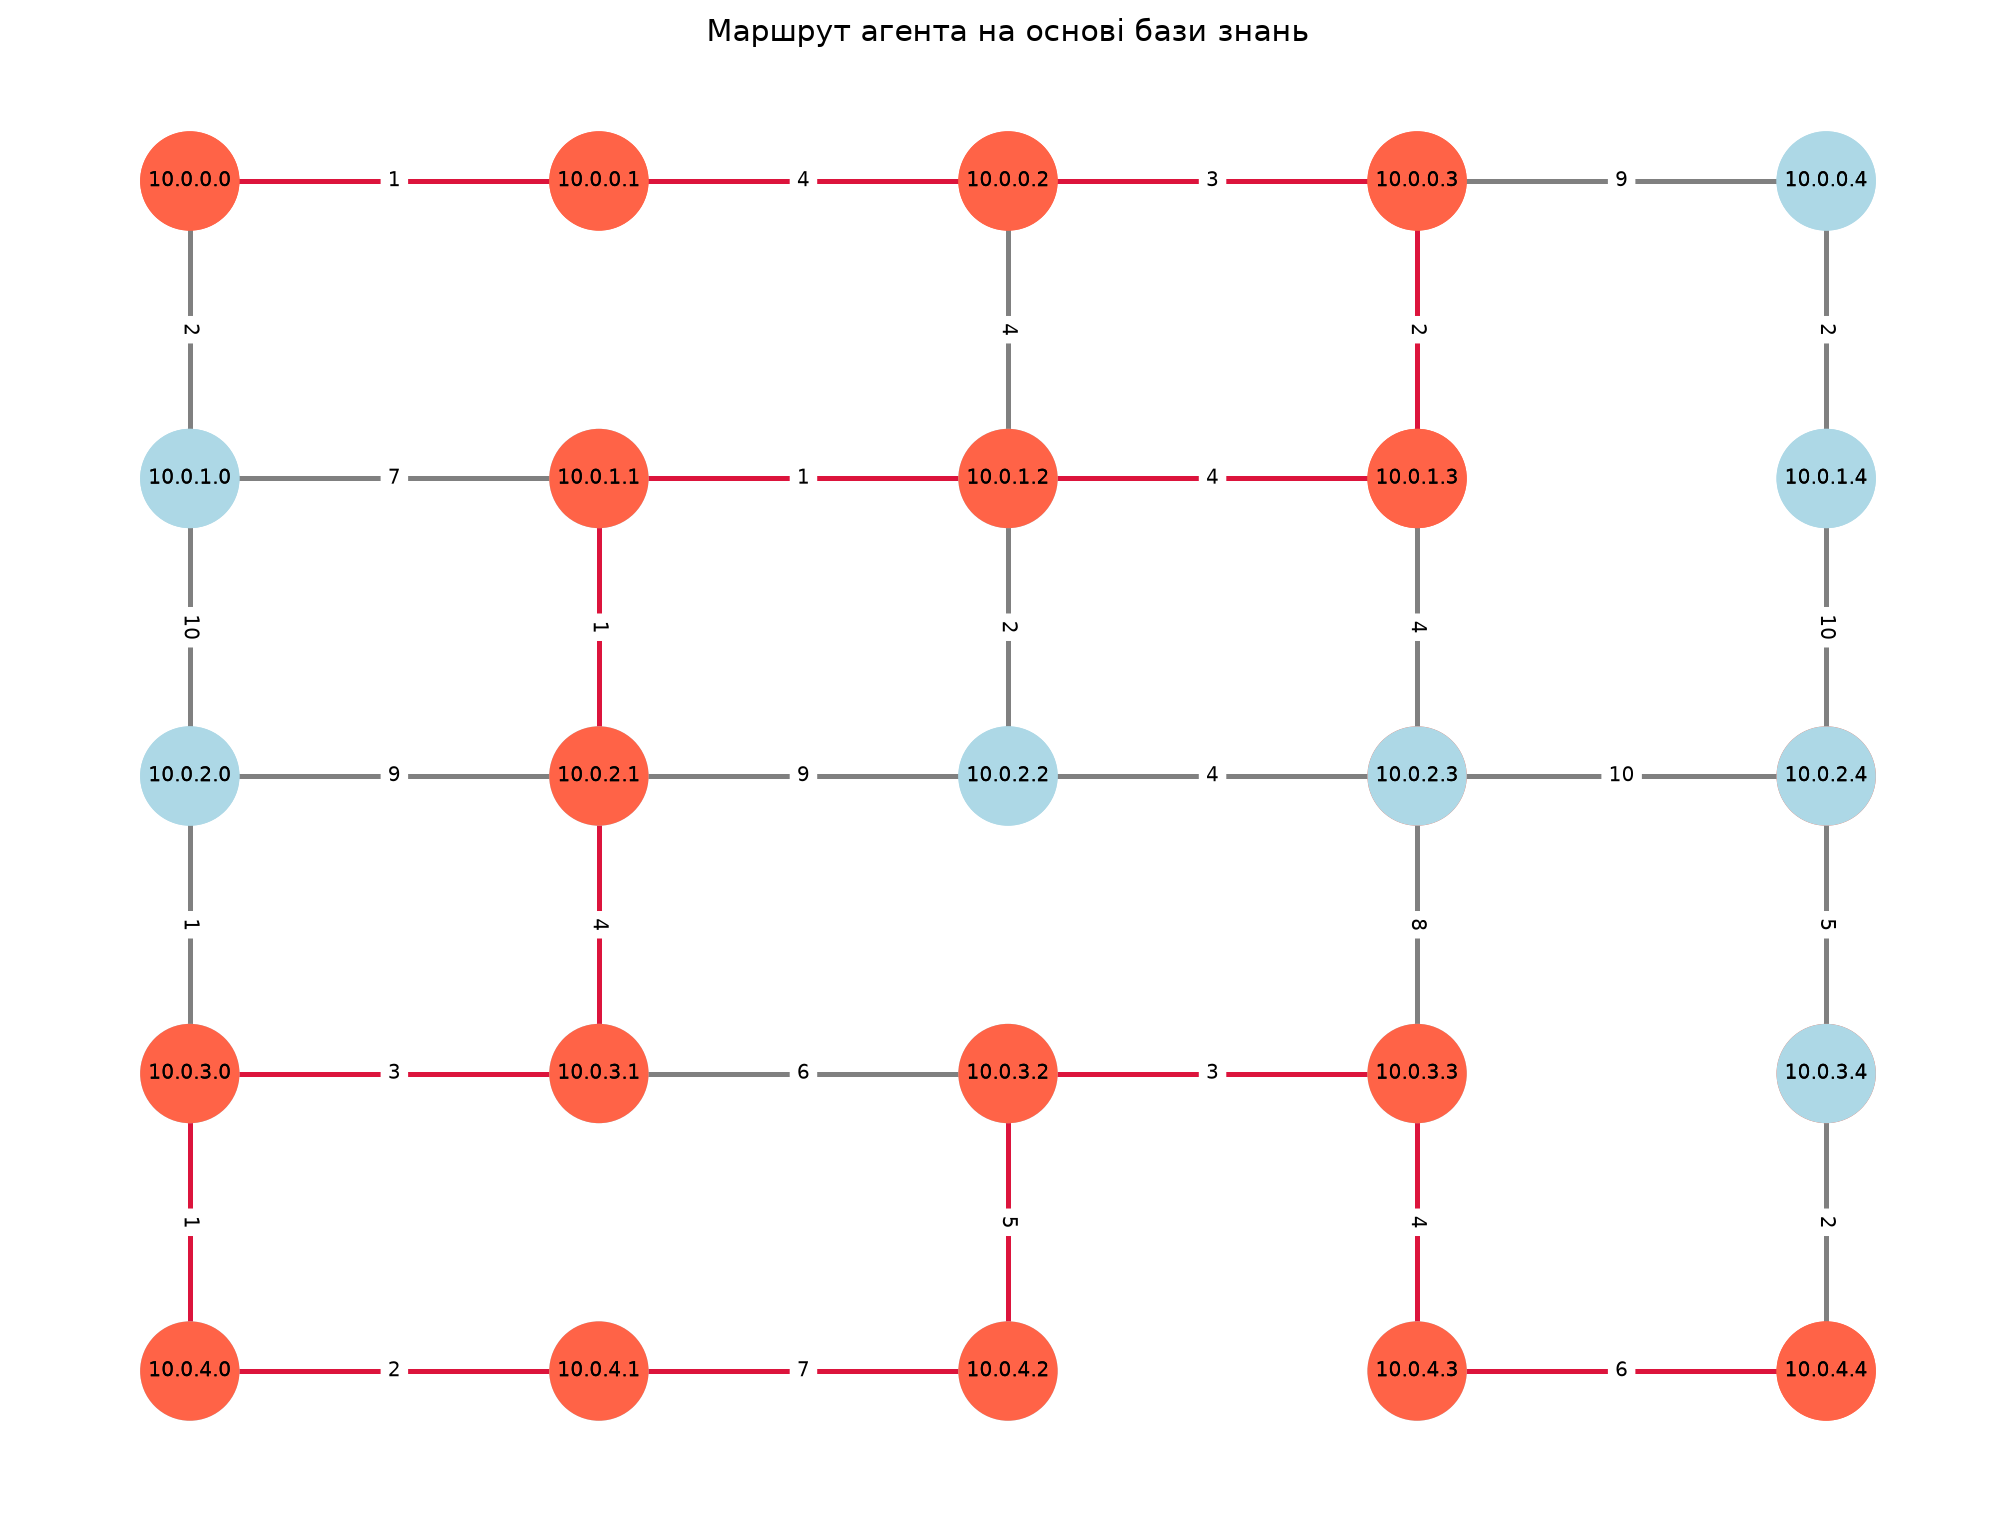
\includegraphics[width=0.94\textwidth]{figures/knowledge_path.png}
  \caption{Маршрут агента на основі бази знань}
\end{figure}

\begin{figure}[H]
  \centering
  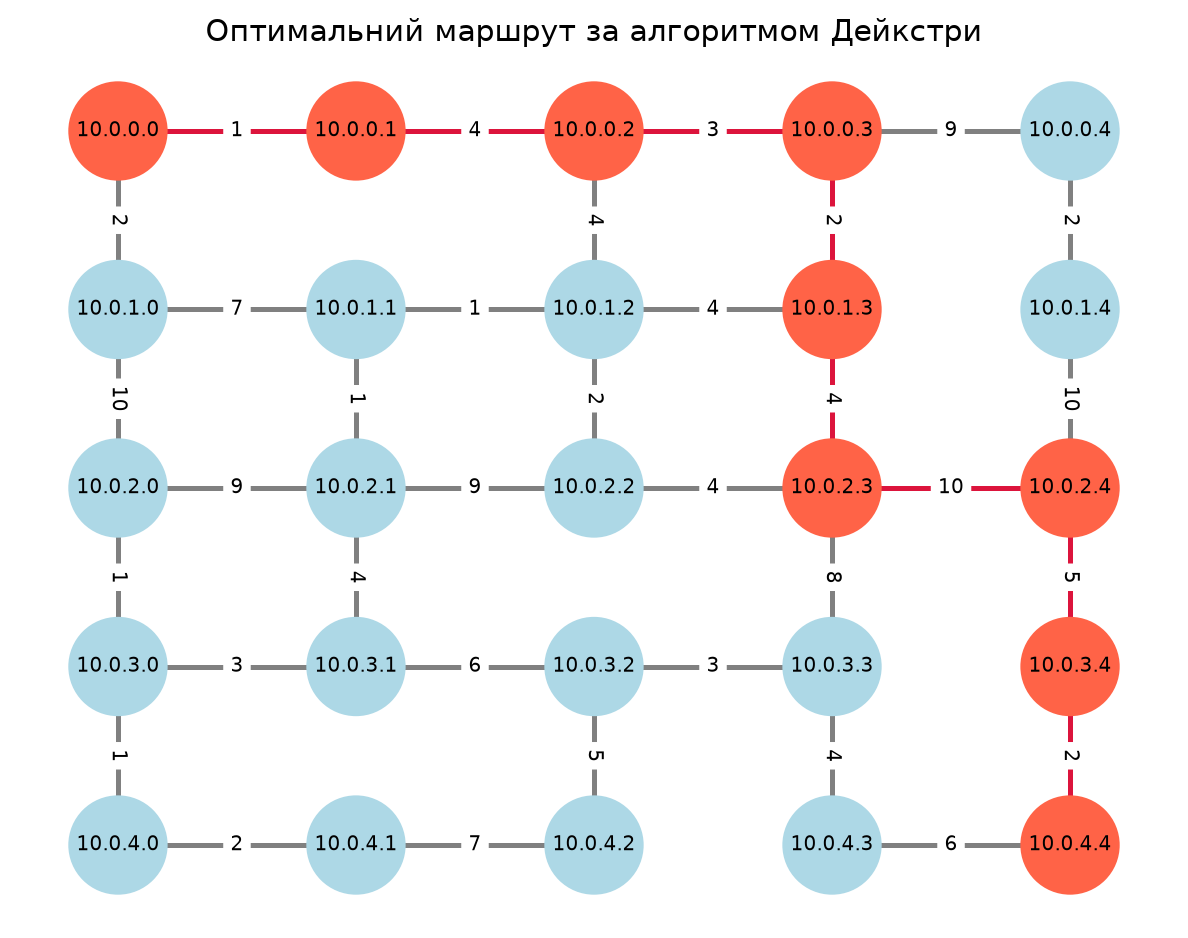
\includegraphics[width=0.94\textwidth]{figures/dijkstra_path.png}
  \caption{Оптимальний маршрут за алгоритмом Дейкстри}
\end{figure}

Для порівняння використано ті самі три топології, що й у лабораторній роботі
№2. У таблиці KBA позначає агента на основі знань.

\begin{table}[H]
\centering
\scriptsize
\resizebox{\textwidth}{!}{%
\begin{tabular}{c r r r r r}
\toprule
{\scriptsize №} & {\scriptsize ЛР2, мс} & {\scriptsize KBA, мс} & {\scriptsize Дейкстра, мс} & {\scriptsize Вузли KBA} & {\scriptsize Відклики KBA}\\
\midrule
1 & 90 & 86 & 40 & 19 & 1\\
2 & 50 & 44 & 38 & 11 & 0\\
3 & 76 & 76 & 35 & 19 & 2\\
\bottomrule
\end{tabular}}
\caption{Порівняння контролерів на однакових топологіях}
\end{table}

У двох із трьох експериментів використання анонсів і бази знань зменшило
сумарну затримку порівняно з агентом ЛР2. У третій топології результат не
змінився, оскільки локальний маршрут уже не потребував додаткового обходу.
В усіх випадках Дейкстра має найменшу затримку, оскільки використовує повний
граф із самого початку.

\section{Висновки}

\small
У лабораторній роботі розроблено агента на основі знань для мережевого
контролера. Агент підтримує базу станів каналів, оновлює її через TELL та
використовує ASK для вибору найкращого відомого маршруту. Експерименти
показали, що накопичення знань зменшує затримку у двох із трьох випадків,
але Дейкстра залишається еталоном завдяки повній інформації про граф.

\appendix
\section{Повний лістинг програми}

Повний програмний код виконаного notebook наведено нижче.

\inputminted{python}{lab3_listing.py}

\end{document}
